% Created 2021-01-17 So 21:18
% Intended LaTeX compiler: pdflatex
\documentclass[11pt]{article}
\usepackage[utf8]{inputenc}
\usepackage[T1]{fontenc}
\usepackage{graphicx}
\usepackage{grffile}
\usepackage{longtable}
\usepackage{wrapfig}
\usepackage{rotating}
\usepackage[normalem]{ulem}
\usepackage{amsmath}
\usepackage{textcomp}
\usepackage{amssymb}
\usepackage{capt-of}
\usepackage{hyperref}
\usepackage{minted}
\usepackage{geometry}\geometry{a4paper,left=15mm,right=20mm,top=20mm,bottom=30mm}
\date{\today}
\title{}
\hypersetup{
 pdfauthor={},
 pdftitle={},
 pdfkeywords={},
 pdfsubject={},
 pdfcreator={Emacs 27.1 (Org mode 9.3)}, 
 pdflang={English}}
\begin{document}

problema:
\begin{center}
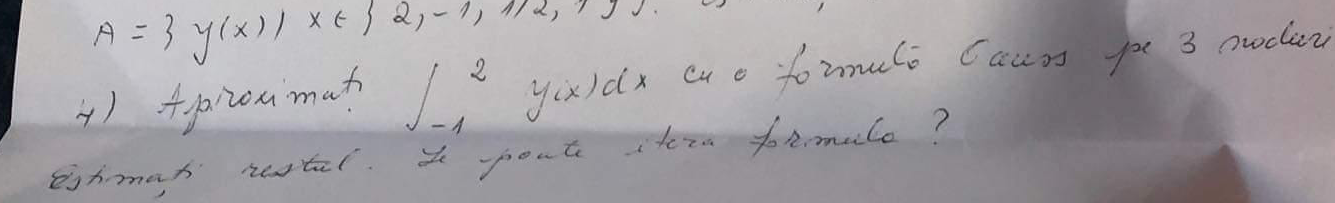
\includegraphics[width=\linewidth]{./problema.png}
\end{center}

BTW, \(y\) de aici e \(y\)-ul aflat la ex 1

avem ponderea \(p(x) = 1\)
\medskip

pentru ca iti cere \(\displaystyle \int y(x) dx \text{ aka } \int y(x) \cdot 1 dx\)\\
daca cerea de ex \(\displaystyle \int e^{-x} y(x) dx\), atunci ponderea era \(e^{-x}\)
\medskip

si cum ponderea e 1, "o formula gauss" inseamna Gauss-Legendre\\
de ex daca era \(e^{-x}\) era gauss-laguerre
\medskip

si acum ar trebui sa convertim functia de la una pe \([-1, 2]\) la una pe \([-1, 1]\) (practic e schimbare de variabila)\\
(Gauss-Legendre cere ca functia sa fie pe intervalul \([-1, 1]\))\\
\url{https://en.wikipedia.org/wiki/Gauss\%E2\%80\%93Legendre\_quadrature}
\medskip

deci folosim:
\begin{center}
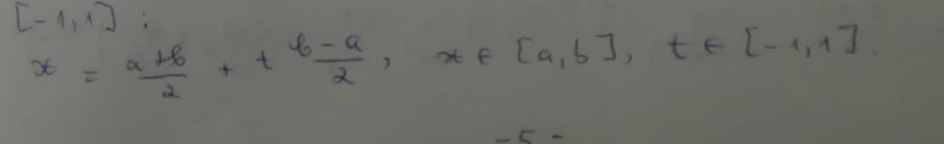
\includegraphics[width=\linewidth]{./a,b to -1,1.png}
\end{center}

formula e
\begin{center}
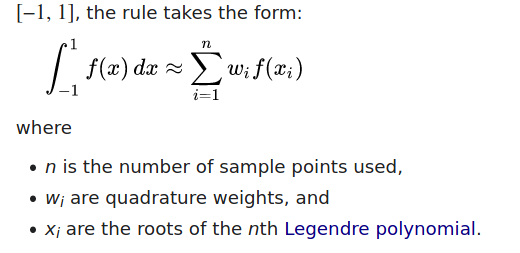
\includegraphics[width=.6\linewidth]{./formula.png}
\end{center}

aici e un tabel pt alte ponderi (am vazut doar ponderea 1 in exercitii)\\
(sau newton cotes- dar asta e alta treaba)\\
\url{https://en.wikipedia.org/wiki/Gaussian\_quadrature}

\begin{center}
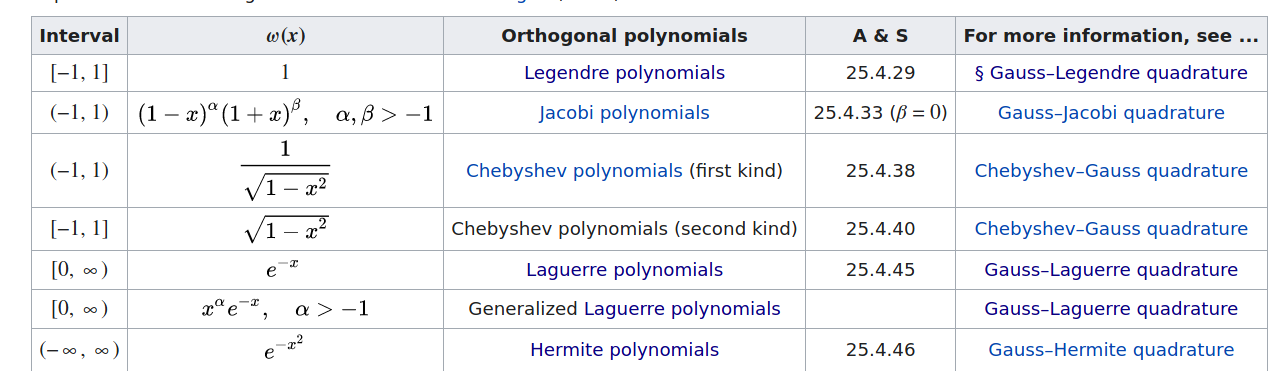
\includegraphics[width=\linewidth]{./table.png}
\end{center}

cum cere pe 3 noduri, \(n = 3\)\\
deci avem nevoie de al 3-lea polinom lagrange - notat de profa cu \(T_3\)
\medskip

pe care-l calculam asa

\begin{center}
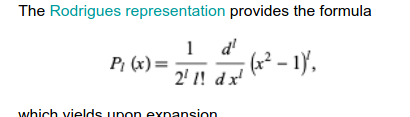
\includegraphics[width=.6\linewidth]{./rodrigues.png}
\end{center}

si ar trebui sa dea atat

\begin{center}
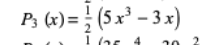
\includegraphics[width=.4\linewidth]{./lagrange3.png}
\end{center}

(sunt mai multe valori aici:\\
\url{https://mathworld.wolfram.com/LegendrePolynomial.html})
\medskip

si trebuie sa afli radacinile polinomului

\medskip
aici are o expresie mai simpla si se vede aproape automat ca radacinile sunt:\\
\(0, \pm \sqrt{5/3}\)

\medskip
deci in formula asta stim \(n =3\), stim \(x_i =\) radacinile, stim functia definita pe \([-1, 1]\)

\begin{center}
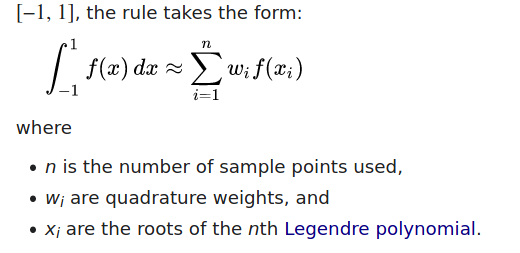
\includegraphics[width=.6\linewidth]{./formula.png}
\end{center}

deci mai avem nevoie doar de \(w_i\)
\medskip

care au minunata forma:

\begin{center}
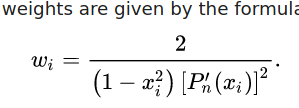
\includegraphics[width=.4\linewidth]{./w_i.png}
\end{center}

cu \(P_n = T_3\) notatia profei\\
adica asta:

\begin{center}
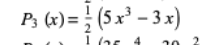
\includegraphics[width=.4\linewidth]{./lagrange3.png}
\end{center}

si acum ai tot ce-ti trebuie, doar inlocuiesti
(si speri la ce e mai bun :))) )
\medskip

si asta e restul:

\begin{center}
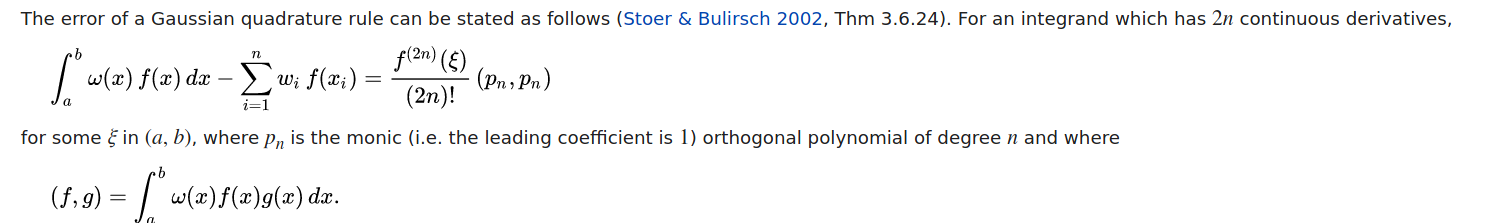
\includegraphics[width=\linewidth]{./rest.png}
\end{center}

aici calculam cu functia pe care am facut-o pe \([-1, 1]\)
si acel \(p_n\) (cred că) e polinomul lagrange la care impartim prin coef lui \(x^3\) (adica \(\frac{5}{2}\)):

\[x^3 - \frac{6}{5} x\]

(de aici
\url{https://en.wikipedia.org/wiki/Gaussian\_quadrature\#Error\_estimates})

\medskip

si acum ultima parte din problema:\\
se poate itera daca \(w_i > 0\), \(\forall i = 1..n\)
\medskip

sanity check:\\
calculeaza integrala (cu wolfram alpha eventual) si verifica daca „seamană” cu ce ti-a dat
\end{document}
